%%%%%%%%%%%%%%%%%%%%%%%%%%%%%%%%%%%%%%%%%%%%%%%%%%%%%%%%%%%%%%%%%%%%%%%%%%%%%%%%
%						GRADIENT VISUALIZATION ON CHAPTER 6 				   %
%%%%%%%%%%%%%%%%%%%%%%%%%%%%%%%%%%%%%%%%%%%%%%%%%%%%%%%%%%%%%%%%%%%%%%%%%%%%%%%%
As a final demonstration of the technique, we now apply \gls{gv} on the trained \glspl{cnn} from the two attacks \attCNN{} described in \autoref{sec:cnn_archi_esorics}, in order to show how this characterization method can provide insights about the acquired traces and the behavior of the target device.
For completeness, we additionnaly trained \glspl{cnn} targeting the remaining bytes of the secret key which have not been investigated yet for the attacks \attCNN{} in \autoref{chap:dl_sca_practice}.
The architecture used for those additional trainings remained exactly the same, namely:
\begin{equation}\label{eq:vgg_archi_esorics_grad}
	\softmax \circ \linLayer_{\card{\sensVarSet}} \circ [\actLayer \circ \linLayer_\linSize]^{n_1}
	\circ [\poolLayer_\pstride \circ \actLayer \circ \BNLayer \circ \convLayer_{\ksize, \numFilters}]^{n_2} \circ \BNLayer \enspace ,
\end{equation}
where \(\convLayer_{\ksize, \numFilters}\) denotes a convolutional layer made of \(\numFilters\) filters of size \(\ksize\), \(\BNLayer\) denotes a batch-normalization layer, \(\actLayer\) denotes the \gls{relu} activation function, \(\poolLayer_{\pstride}\) denotes an average pooling layer of size \(\pstride\), \(\linLayer\) denotes a dense layer, and \(\softmax\) denotes the softmax layer.
The hyper-parameters are given in \autoref{table:cnn_archi}.

\paragraph{\mbedTLS{}}
\autoref{fig:grad_mbed} shows the gradient visualizations applied on one trace from the \mbedTLS{} dataset based on the corresponding trained \gls{cnn}.
The top plot shows a trace whereas the bottom plots show the 16 gradients computed from this trace, targeting each byte.
Those gradients have been gathered into four pools.
\begin{figure}
	\centering
	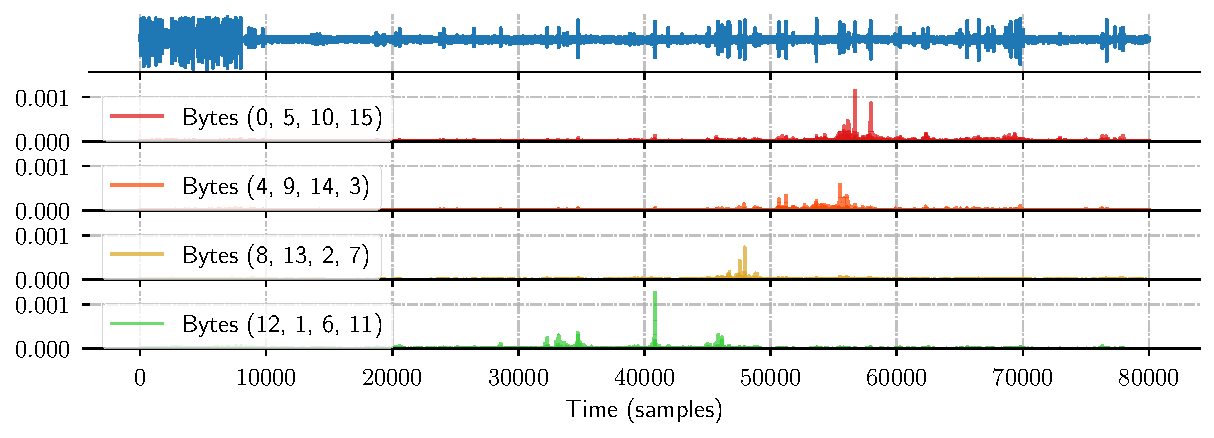
\includegraphics[width=\textwidth]{../Chapter6/Figures/grad_viz/v1/grads}
	\caption{\gls{gv} for one trace of the \mbedTLS{} implementation.}
	\label{fig:grad_mbed}
\end{figure}
First, it can be remarked that contrary to the \gls{snr} plotted in \autoref{fig:observations_v1}, the \gls{gv} shows some peaks in the different gradients plotted in \autoref{fig:grad_mbed}, which shows that the \gls{gv} is able to emphasize the \glspl{poi} despite the application of code polymorphism on the target implementation.

More particularly, it may be seen that the peaks of gradient corresponding to the bytes \((12, 1, 6, 11)\) colored in green appear first, followed by those of the bytes \((8, 13, 2, 7)\) in yellow, then those of the bytes \((4, 9, 14, 3)\) in orange and finally the peaks of gradient for the bytes \((0, 5, 10, 15)\) in red.
Interestingly, this order can be read in light of the source code of the implementation.
The \gls{aes} state is represented here by four \verb+uint32_t+ variables \verb+X0+, 
\ldots, \verb+X3+, each one denoting one column of the state array.
The repartition of the bytes into the state is represented in \autoref{fig:aes_state} at two steps of the first round which could potentially be the leakage source.
\begin{figure}
	\begin{subfigure}{0.49 \textwidth}
		\centering
		\begin{tikzpicture}[scale=0.5]
    \draw[fill=ceared!20] (0,3) rectangle node {\scriptsize 0} +(0.8,1);
    \draw[fill=cealime!20] (0,2) rectangle node {\scriptsize 1} +(0.8,1);
    \draw[fill=ceagold!20] (0,1) rectangle node {\scriptsize 2} +(0.8,1);
    \draw[fill=ceaorange!20] (0,0) rectangle node {\scriptsize 3} +(0.8,1);
    \draw[fill=ceaorange!20] (1,3) rectangle node {\scriptsize 4} +(0.8,1);
    \draw[fill=ceared!20] (1,2) rectangle node {\scriptsize 5} +(0.8,1);
    \draw[fill=cealime!20] (1,1) rectangle node {\scriptsize 6} +(0.8,1);
    \draw[fill=ceagold!20] (1,0) rectangle node {\scriptsize 7} +(0.8,1);
    \draw[fill=ceagold!20] (2,3) rectangle node {\scriptsize 8} +(0.8,1);
    \draw[fill=ceaorange!20] (2,2) rectangle node {\scriptsize 9} +(0.8,1);
    \draw[fill=ceared!20] (2,1) rectangle node {\scriptsize 10} +(0.8,1);
    \draw[fill=cealime!20] (2,0) rectangle node {\scriptsize 11} +(0.8,1);
    \draw[fill=cealime!20] (3,3) rectangle node {\scriptsize 12} +(0.8,1);
    \draw[fill=ceagold!20] (3,2) rectangle node {\scriptsize 13} +(0.8,1);
    \draw[fill=ceaorange!20] (3,1) rectangle node {\scriptsize 14} +(0.8,1);
    \draw[fill=ceared!20] (3,0) rectangle node {\scriptsize 15} +(0.8,1);	

    \draw (0.4,-1) node {\scriptsize \verb+X0+};
    \draw (1.4,-1) node {\scriptsize \verb+X1+};
    \draw (2.4,-1) node {\scriptsize \verb+X2+};
    \draw (3.4,-1) node {\scriptsize \verb+X3+};
\end{tikzpicture}
		\caption{\gls{aes} state after the first \ark{}}
		\label{fig:aes_state_ark}
	\end{subfigure}
	\begin{subfigure}{0.49 \textwidth}
		\centering
		\begin{tikzpicture}[scale=0.5]
    \draw[fill=ceared!20] (0,3) rectangle node {\scriptsize 0} +(0.8,1);
    \draw[fill=ceared!20] (0,2) rectangle node {\scriptsize 5} +(0.8,1);
    \draw[fill=ceared!20] (0,1) rectangle node {\scriptsize 10} +(0.8,1);
    \draw[fill=ceared!20] (0,0) rectangle node {\scriptsize 15} +(0.8,1);
    \draw[fill=ceaorange!20] (1,3) rectangle node {\scriptsize 4} +(0.8,1);
    \draw[fill=ceaorange!20] (1,2) rectangle node {\scriptsize 9} +(0.8,1);
    \draw[fill=ceaorange!20] (1,1) rectangle node {\scriptsize 14} +(0.8,1);
    \draw[fill=ceaorange!20] (1,0) rectangle node {\scriptsize 3} +(0.8,1);
    \draw[fill=ceagold!20] (2,3) rectangle node {\scriptsize 8} +(0.8,1);
    \draw[fill=ceagold!20] (2,2) rectangle node {\scriptsize 13} +(0.8,1);
    \draw[fill=ceagold!20] (2,1) rectangle node {\scriptsize 2} +(0.8,1);
    \draw[fill=ceagold!20] (2,0) rectangle node {\scriptsize 7} +(0.8,1);
    \draw[fill=cealime!20]  (3,3) rectangle node {\scriptsize 12} +(0.8,1);
    \draw[fill=cealime!20] (3,2) rectangle node {\scriptsize 1} +(0.8,1);
    \draw[fill=cealime!20] (3,1) rectangle node {\scriptsize 6} +(0.8,1);
    \draw[fill=cealime!20] (3,0) rectangle node {\scriptsize 11} +(0.8,1);	

    \draw (0.4,-1) node {\scriptsize \verb+X0+};
    \draw (1.4,-1) node {\scriptsize \verb+X1+};
    \draw (2.4,-1) node {\scriptsize \verb+X2+};
    \draw (3.4,-1) node {\scriptsize \verb+X3+};
\end{tikzpicture}
		\caption{\gls{aes} state at the end of the \sr{}}
		\label{fig:aes_state_mc}
	\end{subfigure}
	\caption{\gls{aes} states at two moments in the first round potentially leaking information about the secret key bytes.}
	\label{fig:aes_state}
\end{figure}
\autoref{fig:aes_state_ark} denotes the state after the first \ark{} while \autoref{fig:aes_state_mc} denotes the state at the end of the \sr{}.
Since the operations are done column-wise, the bytes belonging to the same column of the state should leak at close time samples to each other in the trace.
That being said, we easily remark that the pools of gradient peaks described above coincide with the columns of the \gls{aes} state at the end of the \sr{} depicted in \autoref{fig:aes_state_mc}, which corresponds to the call of the \glspl{lut} of the T-table implementation, rather than the key addition.

\paragraph{\aeshuitbit{}}
\begin{figure}
	\centering
	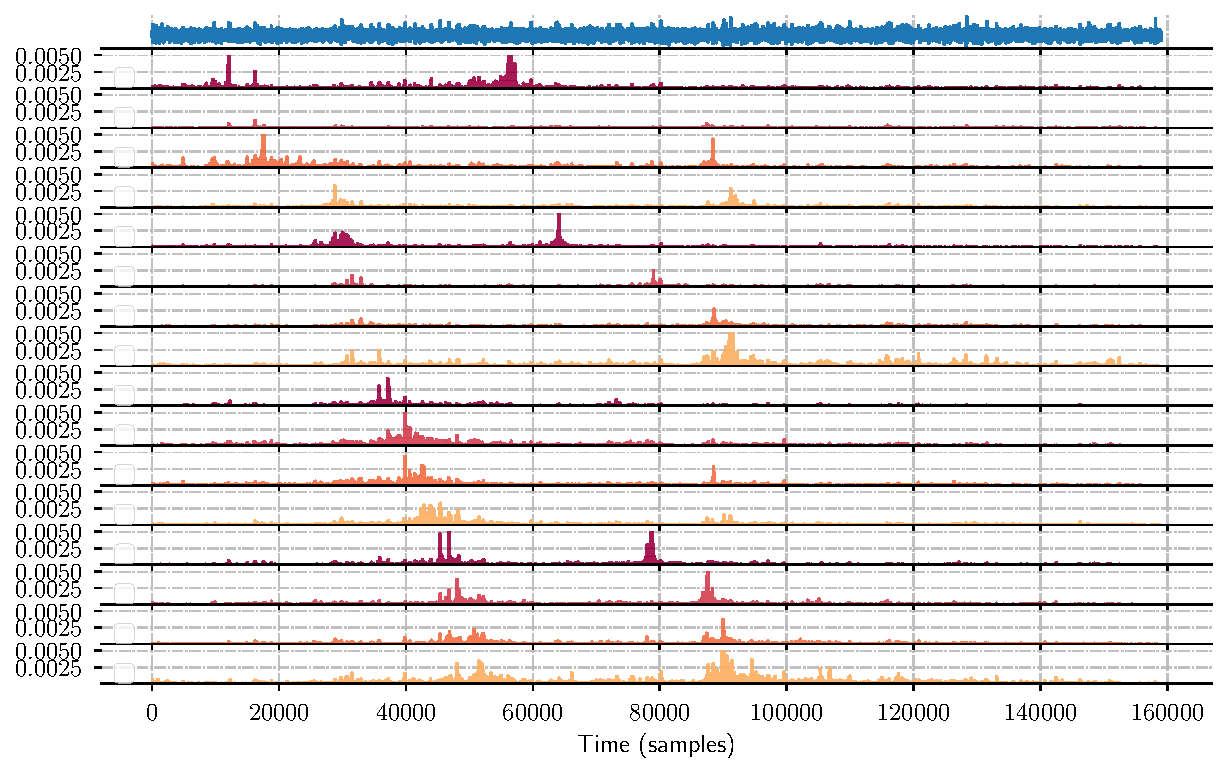
\includegraphics[width=\textwidth]{../Chapter6/Figures/grad_viz/v2/grads}
	\caption{\gls{gv} for one trace of the \aeshuitbit{} implementation.
	The top plot depicts the considered trace, whereas the bottom plots denote
	the gradients for each targeted byte.}
	\label{fig:grad_aes8bit}
\end{figure}
\autoref{fig:grad_aes8bit} shows the gradient visualizations in the same way as for \mbedTLS{}, but this time, for each key byte separately.
A focus on the first peak of each gradient highlights that they appear in increasing order of the byte index: the leakage probably comes from a \verb+for+ loop iterating over each byte of the \gls{aes} state.
Thus, the corresponding operation might be either \ark{} or \sub{}.
Furthermore, a close look at the second peak of each gradient reveals that they are almost aligned, except four of them: \((0, 4, 8, 12)\).
A quick look at the \sr{} operation inside the source code of the \aeshuitbit{} implementation reveals that it never manipulates the latter bytes of the state, contrary to the others.
This can also be deduced from \autoref{fig:aes_state} where the only bytes not moving from \autoref{fig:aes_state_ark} to \autoref{fig:aes_state_mc} are those same bytes.
We deduce that for the bytes \(0, 4, 8, 12\), the \gls{cnn} exploits the joint leakages of the \ark{} and \sub{} operations, whereas for the other bytes the \gls{cnn} rather exploits the joint leakages of the \ark{} and \sr{} operations.

Anyway, in every cases, two leakages are jointly exploited by the \gls{cnn} in the \aeshuitbit{} implementation whereas only one leakage seems to be used in the \mbedTLS{} one.
This might explain why the attack on the latter implementation is slightly worse than in the former implementation, although the traces seemed less noisy at first sight. 

Finally, the gradient visualizations showed in both \autoref{fig:grad_mbed} and \autoref{fig:grad_aes8bit} highlight relatively sharp peaks.%
\footnote{A similar analysis can be done on other traces from the dataset.}
This means that the \gls{cnn} model is able to precisely localize the leakages in the traces, despite the application of code polymorphism.
In other words, the code transformations applied here did not prevent the \gls{cnn} model to localize and exploit the leakage.
Instead, one would expect sound code transformations to flatten and spread the gradient peaks along a wider zone of the trace, in order to increase uncertainty about the leakage localization.
One might imagine other code transformations which could be plugged in the Belleville \etal{}'s tool in order to address this problem, although beyond the scope of this demonstration.